\documentclass[serif,xcolor=pdftex,dvipsnames,table,hyperref={bookmarks=false,breaklinks}]{beamer}

%%%%%%%%%%%%%%%%
% Change the macros below to configure the title slides
% for your course.
\newcommand{\coursename}{COMPSCI 590N}
\newcommand{\instructor}{Roy J. Adams}
\newcommand{\university}{University of Massachusetts Amherst}
\newcommand{\department}{College of Information and Computer Sciences}
%%%%%%%%%%%%%%%%

\newcommand\HUGE{\@setfontsize\Huge{50}{60}}

\newcommand{\settitlecard}[2]{
  \title[\coursename  Lecture #1] 
    {\coursename \\ Lecture #1: #2}
     \author[\instructor]{\instructor}
     \institute[\university]{
     \department\\
     \university
   }
\date{}
}

\newcommand{\maketitlepage}{
  \begin{frame}
  \titlepage
  %\center{
    %If you use the slides unmodified, retain the attribution below
  %  \tiny{Slides by Roy J. Adams (rjadams@cs.umass.edu). 
    %If you modify the slides, please retain the alternate attribution below
    %\tiny{Based on slides by Roy J. Adams (rjadams@cs.umass.edu). \\    
  %  }                                              
  %}  
  \end{frame}
}

\AtBeginSection[]
{
  \begin{frame}<beamer>{Outline}
    \tableofcontents[currentsection,subsectionstyle=hide]
  \end{frame}
}


\newcommand{\cut}[1]{}

\newcommand{\iconbox}[4]{
  \only<#1-#2>{
    \begin{columns}[T]
      \column{0.5in}
           \includegraphics[width=0.5in]{#3}
       \column{3.7in}
            #4
    \end{columns}
    \medskip
    \medskip
    \medskip
  }
}

\mode<presentation>{
  \usepackage{../beamertheme589theme}
  \setbeamercovered{invisible}
}

\mode<handout>{
  \usepackage{../beamertheme589theme}
  \setbeamercovered{transparent}
}


\usepackage[english]{babel}
\usepackage[latin1]{inputenc}
\usepackage{times}
\usepackage[T1]{fontenc}
\usepackage{amsmath}
\usepackage{amssymb}
\usepackage[noend]{algorithmic}
\usepackage{algorithm}
\usepackage{listings}
\usepackage{tcolorbox}
\usepackage{xmpmulti}

\renewcommand\mathfamilydefault{\rmdefault}

\newcommand{\setA}{\mathcal{A}}
\newcommand{\setB}{\mathcal{B}}
\newcommand{\setS}{\mathcal{S}}
\newcommand{\setV}{\mathcal{V}}
\DeclareMathOperator*{\union}{\bigcup}
\DeclareMathOperator*{\intersection}{\bigcap}
\DeclareMathOperator*{\Val}{Val}
\newcommand{\mbf}[1]{{\mathbf{#1}}}
\DeclareMathOperator*{\argmax}{arg\,max}
\DeclareMathOperator*{\argmin}{arg\,min}
\DeclareMathOperator*{\sign}{sign}
\newcommand{\deriv}[2]{\frac{\partial{#1}}{\partial{#2}}}

\lstdefinestyle{custompython}{
  belowcaptionskip=1\baselineskip,
  breaklines=true,
  frame=single,
  xleftmargin=\parindent,
  language=Python,
  showstringspaces=false,
  basicstyle=\footnotesize\ttfamily,
  keywordstyle=\bfseries\color{green!40!black},
  commentstyle=\itshape\color{purple!40!black},
  identifierstyle=\color{blue},
  stringstyle=\color{orange},
}
\lstset{style=custompython}

\makeatletter
\renewcommand*\env@matrix[1][*\c@MaxMatrixCols c]{%
  \hskip -\arraycolsep
  \let\@ifnextchar\new@ifnextchar
  \array{#1}}
\makeatother

\newcommand\norm[1]{\left\lVert#1\right\rVert}


\settitlecard{7}{Complexity and Numerical Linear Algebra 1}

\begin{document}

\maketitlepage

% \section{Announcements}
% \subsection{Foo}
%
% \begin{frame}[t]{Announcements}
% 	\begin{itemize}
% 		\item Assignment 3 is due on Thursday.
% 	\end{itemize}
% \end{frame}

\section{Assignment 2}
\subsection{Foo}

\begin{frame}[t]{Problem 1}
	\centering
	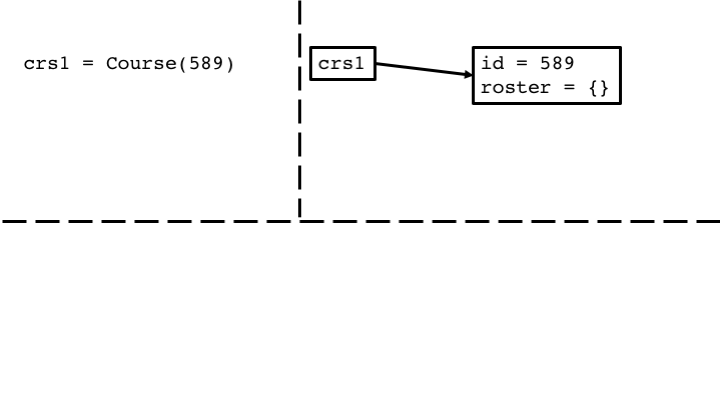
\includegraphics[width=\textwidth]{{../Figures/array_slicing/Slide23}.png}
\end{frame}

\begin{frame}[t]{Problem 1}
	\centering
	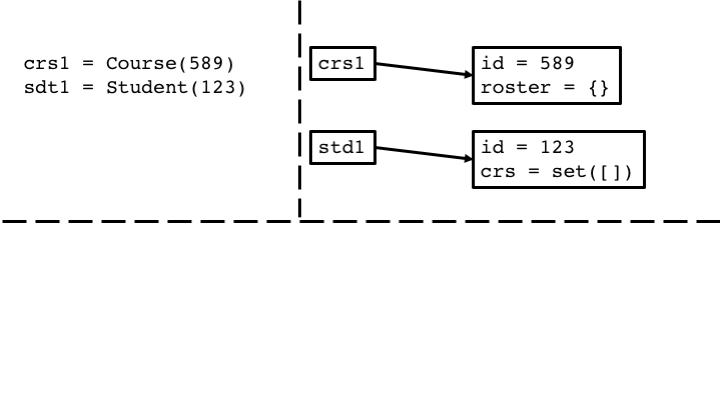
\includegraphics[width=\textwidth]{{../Figures/array_slicing/Slide24}.png}
\end{frame}

\begin{frame}[t]{Problem 1}
	\centering
	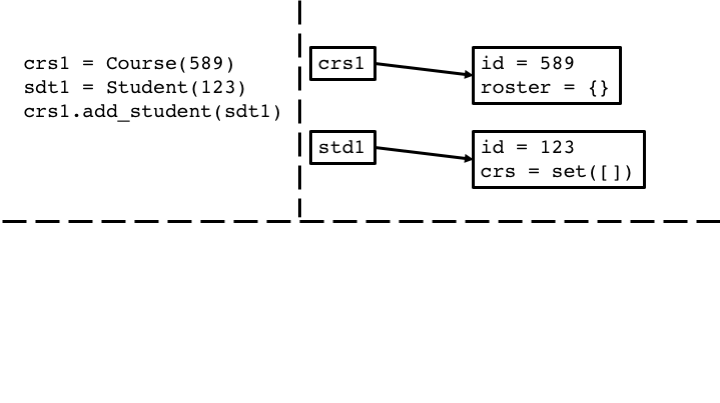
\includegraphics[width=\textwidth]{{../Figures/array_slicing/Slide25}.png}
\end{frame}

\begin{frame}[t]{Problem 1}
	\centering
	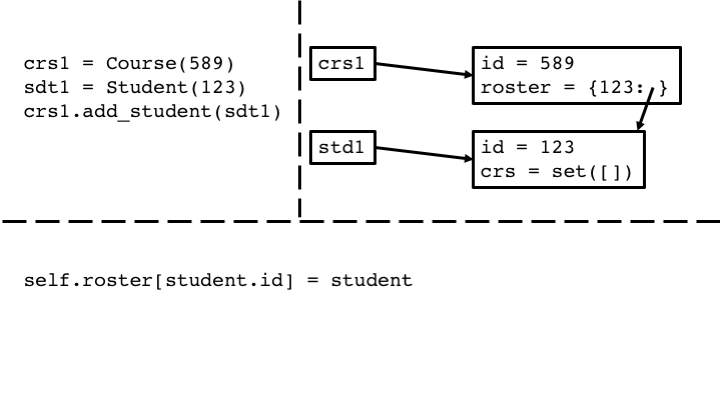
\includegraphics[width=\textwidth]{{../Figures/array_slicing/Slide26}.png}
\end{frame}

\begin{frame}[t]{Problem 1}
	\centering
	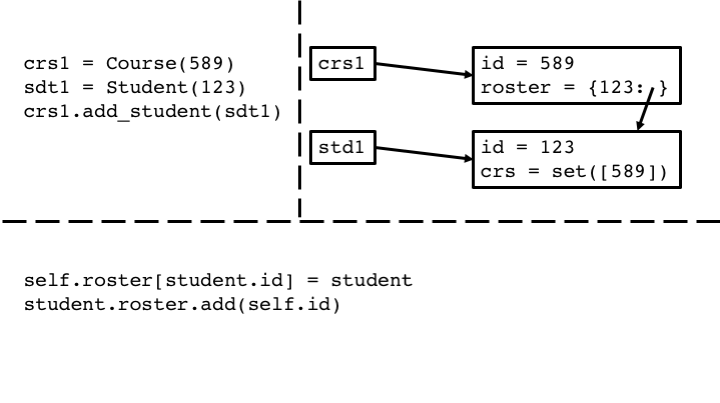
\includegraphics[width=\textwidth]{{../Figures/array_slicing/Slide27}.png}
\end{frame}

\begin{frame}[t]{Problem 1}
	\centering
	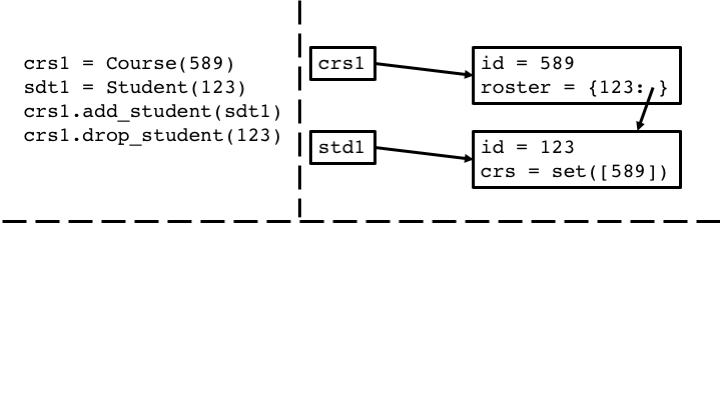
\includegraphics[width=\textwidth]{{../Figures/array_slicing/Slide28}.png}
\end{frame}

\begin{frame}[t]{Problem 1}
	\centering
	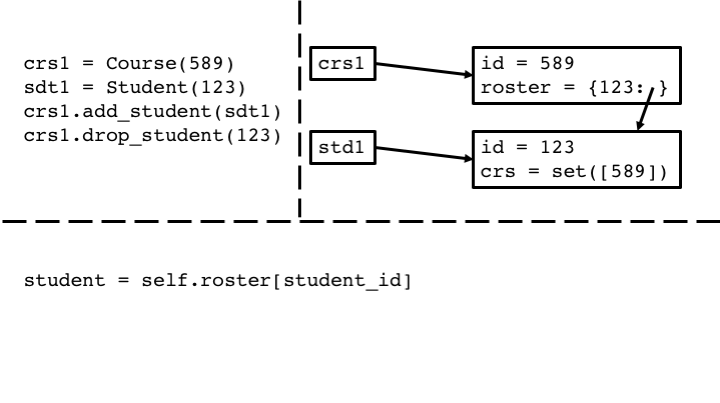
\includegraphics[width=\textwidth]{{../Figures/array_slicing/Slide29}.png}
\end{frame}

\begin{frame}[t]{Problem 1}
	\centering
	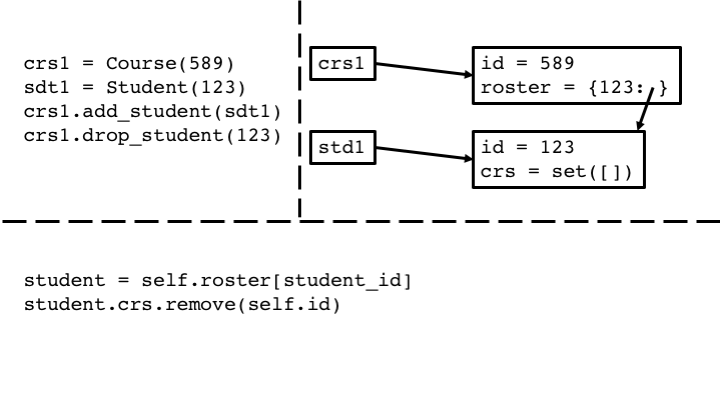
\includegraphics[width=\textwidth]{{../Figures/array_slicing/Slide30}.png}
\end{frame}

\begin{frame}[t]{Problem 1}
	\centering
	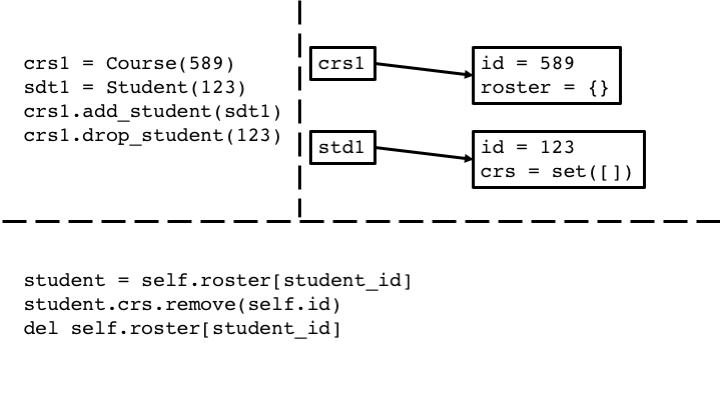
\includegraphics[width=\textwidth]{{../Figures/array_slicing/Slide31}.png}
\end{frame}

\section{NumPy Views}
\subsection{Foo}

\begin{frame}[t,fragile]{Views}
	A \verb|view| of an array is another \verb|ndarray| object that shares the same underlying memory locations.
	
	\pause
	\begin{lstlisting}
		>>> A = np.ones((4,5))
		>>> B = A.view()
		>>> B is A
		False
		>>> B.base is A
		True
	\end{lstlisting}
	
	\pause
	\begin{itemize}[<+->]
		\item \verb|A| and \verb|B| are not the same object, hence \verb|A is B| returns \verb|False|.
		\item The attribute \verb|base| points to the array from which a view was created, hence \verb|B.base is A| returns \verb|True|.
	\end{itemize}
\end{frame}

\begin{frame}[t]{Views}
	Many functions will try to create views if they can, \textbf{but will silently create copies if they can't.} Examples of such operations/functions are:
	\pause
	\begin{itemize}[<+->]
		\item Slicing
		\item transpose
		\item reshape
	\end{itemize}
\end{frame}

\begin{frame}[t,fragile]{Views}
	\begin{lstlisting}
		>>> A = np.ones((4,5))
		>>> B = A.transpose()
		>>> B.base is A
		True
		>>> C = B.reshape((5,4)) # Creates another view
		>>> C.base is A
		True
		>>> D = B.reshape((2,10)) # Creates a copy!
		>>> D.base is A
		False
	\end{lstlisting}
\end{frame}
	
\begin{frame}[t]{Views}
	\begin{itemize}[<+->]
		\item There are rules for when a view will be made, however, they are not well documented and rely on an understanding of the underlying storage.
		\item The moral of the story is: be careful when modifying the contents of an array directly.
		\item When in doubt, create a copy!
	\end{itemize}
\end{frame}

\section{Computational Complexity}
\subsection{Foo}

\begin{frame}[t]{Computational Complexity}
	\begin{itemize}[<+->]
		\item In our discussion of numerical algorithms so far, we have obliquely discussed the speed of our algorithms. 
		\item We need a formal language for discussing the speed of an algorithm.
		\item The mathematical language used by computer scientists and mathematicians is called \emph{complexity}.
	\end{itemize}
\end{frame}

\begin{frame}[t]{Computational Complexity}
	High level idea: The complexity of an algorithm is the number of \emph{basic operations} used by the algorithm as a function of the input size.
	
	\pause
	\begin{block}{Basic operations}
		A basic operation is any computation that has a constant runtime as a function of the input size. Think of basic operations as the building blocks of algorithms.
	\end{block}
	
	\pause
	Examples include: arithmetic operations, basic functions, logical comparisons, basic indexing, and assignment.
\end{frame}

\begin{frame}[t,fragile]{Array Scanning}
	Let's consider an example: Finding the maximum value in a list of numbers.
	
	\pause
	\begin{lstlisting}
		def max(A):
		    m = -inf
		    for a in A:
		        if a > m:
		            m = a
		    return m
	\end{lstlisting}
	
	\pause
	\begin{itemize}[<+->]
		\item What are the basic operations used in this algorithm?
		\item If \verb|A| has length $n$, how many basic operations will be performed by \verb|max|?
		\item Aside from $n$, does the run time of \verb|max| depend on the contents of \verb|A|?
	\end{itemize}
\end{frame}

\begin{frame}[t,fragile]{Worst case analysis}
	In the previous, example, \verb|max| didn't depend on the contents of \verb|A| beyond its size. This is not always the case.
	
	\pause
	\begin{lstlisting}
		def find_first_zero(A):
		    i = 0
		    for a in A:
		        if a == 0:
		            return i
		        else:
		            i += 1
		    return None
	\end{lstlisting}
	
	\pause
	\begin{itemize}[<+->]
		\item What are the basic operations used in this algorithm?
		\item If \verb|A| has length $n$, how many basic operations will be performed by \verb|find_first_zero|?
		\item It is standard practice to assume the worst possible contents of \verb|A|. This is called \textbf{worst-case analysis}.
	\end{itemize}
\end{frame}

\begin{frame}[t,fragile]{Binary Search}
	Problem: Given a \textbf{sorted} list of unique numbers, \verb|A|, and a number of interest, \verb|x|, find the position of \verb|x| in \verb|A|. Return \verb|None| if \verb|x| is not in \verb|A|.
	
	\pause
	\begin{lstlisting}
		def linear_search(A,x):
		    i = 0
		    for a in A:
		        if a == x:
		            return i
		        else:
		            i += 1
		    return None
	\end{lstlisting}
	
	\pause
	\begin{itemize}[<+->]
		\item What is the worst case?
		\item If \verb|A| has length $n$, what is the worst case number of operations performed by \verb|linear_search|?
		\item What information is not being used by \verb|linear_search|?
	\end{itemize}
	
\end{frame}

\begin{frame}[t]{Binary Search}
	Instead, we can use a more sophisticated algorithm called \textbf{binary search}.
	
	% Insert image
	\pause
	\begin{block}{Binary Search: Basic Idea}
		\begin{itemize}[<+->]
			\item Look at the item in the middle of the list, call this item $m$. 
			\item We know that everything before $m$ is less than $m$ and everything after is greater than $m$.
			\item Therefore, if $x > m$, we can eliminate the first half of the list and if $x < m$ we can eliminate the second half.
			\item Apply this idea recursively.
		\end{itemize}
	\end{block}
	
\end{frame}

\begin{frame}[t]{Binary Search}
	\centering
	\Huge{Animation}
\end{frame}

\begin{frame}[t,fragile]{Binary Search}
	The following code implements binary search in Python.
	
	\pause
	\begin{lstlisting}
		def binary_search(A,x):
		    cur_min_idx = 0
		    cur_max_idx = len(A) - 1
		    while cur_min_idx <= cur_max_idx:
		        cur_split = cur_min_idx + np.floor((cur_max_idx - cur_min_idx)/2)
		        if A[cur_split] > x:
		            cur_min_idx = cur_split + 1
		        elif A[cur_split] < x:
		            cur_max_idx = cur_split - 1
		        else:
		            return cur_split
		    return None
	\end{lstlisting}
\end{frame}
	
\begin{frame}[t,fragile]{Binary Search}
	\begin{itemize}[<+->]
		\item What is the worst case?
		\item If \verb|A| has length $n$, what is the worst case number of operations performed by \verb|binary_search|?
		\begin{itemize}[<+->]
			\item In each iteration, we are dividing the list in half so \verb|binary_search| will take $\log(n)$ iterations.
		\end{itemize}
	\end{itemize}
\end{frame}

\begin{frame}[t]{Big O Notation}
	Computer scientists and mathematicians have a formal notation for discussing the run time of an algorithm as a function of the algorithm's input size.
	
	\pause
	\begin{block}{Big O Notation}
		Let $f$ and $g$ be functions, then $f(x) = \mathcal{O}(g(x))$ if and only if there exists a constant $M$ and $x_0$ such that
		
		$$|f(x)| \leq M|g(x)| \text{ for all } x \geq x_o$$
		
		Intuitively, this means that for large numbers $g(x)$ is always greater than $f(x)$, up to a constant.
	\end{block}
\end{frame}

\begin{frame}[t]{Big O Notation}
	% image
	\centering
	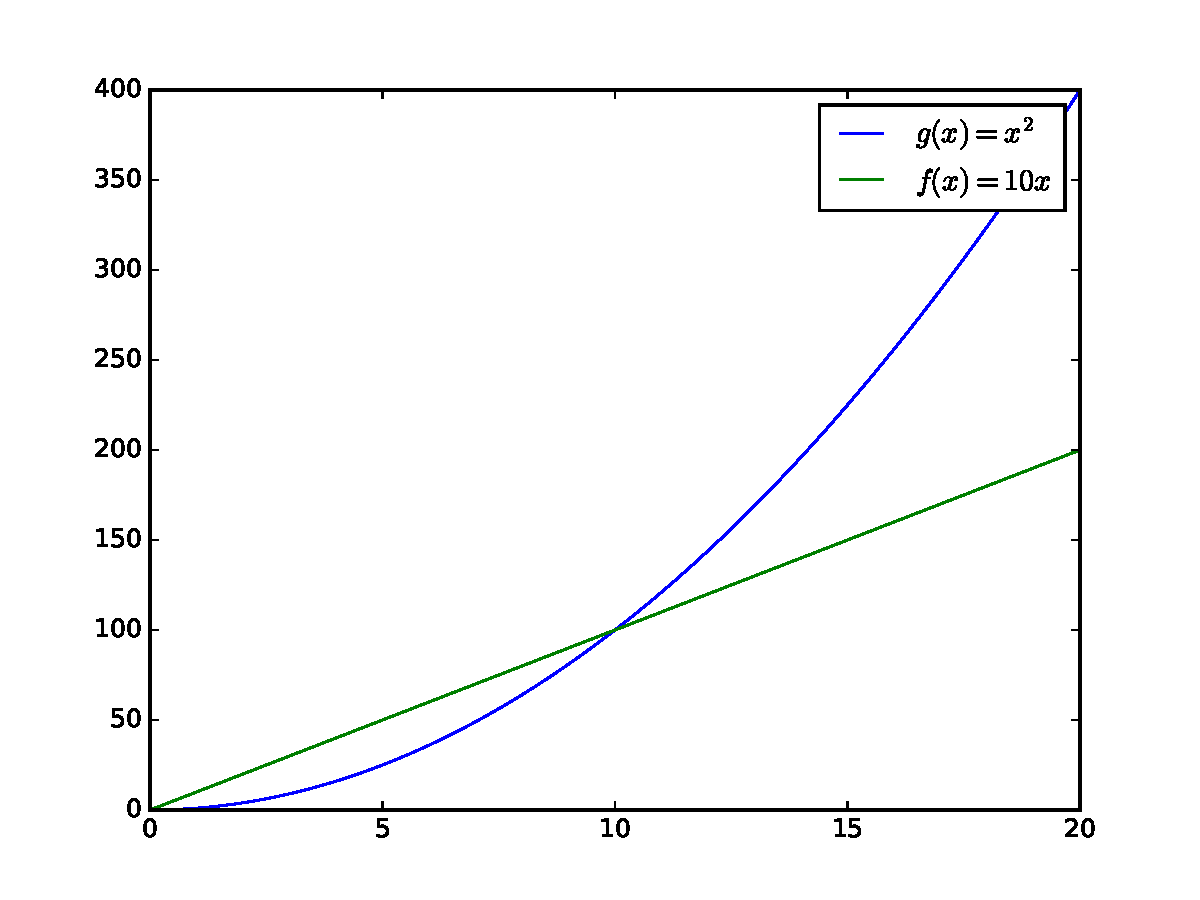
\includegraphics[height=2.5in]{{../Figures/big_o}.pdf}
\end{frame}

\begin{frame}[t]{Takeaways}
	\begin{itemize}[<+->]
		\item An algorithm's \textbf{complexity} is a measure of its run-time as a function of the input size, ignoring constant factors.
		\item It is typical to consider the \textbf{worst-case} input of a fixed size.
		\item Big-O notation is used to formalize this concept so that algorithms can be rigorously compared.
	\end{itemize}
\end{frame}

\section{Numerical Linear Algebra}
\subsection{Foo}

\begin{frame}[t]{Intro}
	% What is numerical linear algebra
	% What are the high level problems in NLA?
	\begin{itemize}[<+->]
		\item Numerical Linear Algebra is the study of efficient algorithms for performing linear algebra computations.
		\item Linear algebra computations are at the core \textbf{many} algorithms. For example:
		\begin{itemize}[<+->]
			\item Linear regression uses matrix multiplication and inversion.
			\item PageRank, the algorithm that spawned Google, was fundamentally calculating eigenvalues.
			\item Many of the recommendation systems that power sites like Netflix, Amazon, Google Ads, etc. are based on matrix decomposition.
		\end{itemize}
	\end{itemize}
\end{frame}

\begin{frame}[t,fragile]{Element-wise Operations}
	\begin{itemize}[<+->]
		\item The most basic operations we have discussed are element-wise operations.
		\item Example: What is the complexity of multiplying an $n\times n$ matrix by a scalar?
	\end{itemize}
	
	\pause
	\begin{lstlisting}
		Input: A, alpha
		Output: B
		for i in 1,...,n:
		    for j in 1,...,n:
		        B[i,j] = alpha*A[i,j]
	\end{lstlisting}
	
	\pause
	Scalar/matrix operations have complexity $\mathcal{O}(n^2)$ for an $n\times n$ matrix.
\end{frame}

\begin{frame}[t,fragile]{Element-wise Operations}
	\begin{itemize}[<+->]
		\item What about matrix addition?
	\end{itemize}
	
	\pause
	\begin{lstlisting}
		Input: A, B
		Output: C
		for i in 1,...,n:
		    for j in 1,...,n:
		        C[i,j] = A[i,j] + B[i,j]
	\end{lstlisting}
	
	\pause
	Element-wise matrix/matrix operations have complexity $\mathcal{O}(n^2)$ for two $n\times n$ matrices.
\end{frame}

\begin{frame}[t,fragile]{Inner Products}
	\begin{itemize}[<+->]
		\item A useful skill for evaluating numerical algorithms is translation between sums/products and loops. 
		\item Take for example the inner product of two length $n$ vectors, $x$ and $y$.
	\end{itemize}
	%
	\pause
	$$x^Ty = \sum_i x_i y_i$$
	%
	\pause
	\begin{lstlisting}
		Input: x, y
		Output: out
		out = 0
		for i in 1,...,n:
		    out += x[i]*y[i]
	\end{lstlisting}
	%
	\pause
	A single sum/product can often be translated directly to a loop. This means that the inner product of two length $n$ vectors has complexity $\mathcal{O}(n)$
	
\end{frame}

\begin{frame}[t,fragile]{Outer Products}
	Outer products, on the other hand, contain no sums. Instead, the output is an $n\times n$ matrix.
	%
	\pause
	$$A = xy^T \text{ s.t. } A_{ij} = x_i y_j$$
	%
	\pause
	\begin{lstlisting}
		Input: x, y
		Output: A
		out = 0
		for i in 1,...,n:
		    for j in 1,...,n:
		        A[i,j] = x[i]*y[j]
	\end{lstlisting}
	%
	\pause
	Outer products have complexity $\mathcal{O}(n^2)$.

\end{frame}

\begin{frame}[t,fragile]{Matrix Multiplication}
	Matrix multiplication can be decomposed into a bunch of vector products. Let $A$ and $B$ be $n \times n$ matrices, then
	
	\pause
	$$C = AB \text{ s.t. } C_{ij} = A_{i:} B_{:j} = \sum_k A_{ik}B_{kj}$$
	
	\pause
	\begin{lstlisting}
		Input: A, B
		Output: C
		for i in 1,...,n:
		    for j in 1,...,n:
		        C[i,j] = 0
		        for k in 1,...,n:
		            C[i,j] += A[i,k]*B[k,j]
	\end{lstlisting}

	\pause
	The naive method for matrix multiplication has complexity $\mathcal{O}(n^3)$.
\end{frame}

\begin{frame}[t]{Strassen's Algorithm}
	Modern linear algebra libraries actually use more advanced matrix multiplication algorithms based on \textbf{Strassen's Algorithm}.
	
	\pause
	\begin{block}{Strassen's Algorithm: Basic Idea}
		\begin{itemize}[<+->]
			\item The naive matrix multiplication method requires 8 operations to multiply $2 \times 2$ matrices, however, Strassen found a way to do it in 7 operations at higher cost per operation. 
			\item Strassen's algorithm recursively divides a matrix into $2 \times 2$ matrices and applies Strassen's $2 \times 2$ method.
		\end{itemize}
	\end{block}
\end{frame}

\begin{frame}[t]{Strassen's Algorithm}
	% Strassen illustration
	\centering
	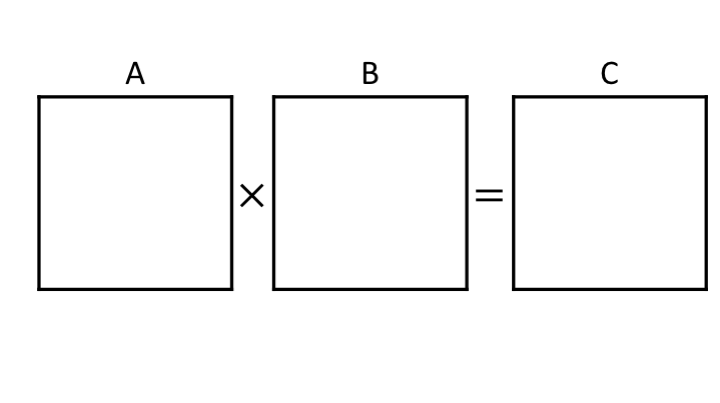
\includegraphics[width=\textwidth]{{../Figures/array_slicing/Slide17}.png}
\end{frame}

\begin{frame}[t]{Strassen's Algorithm}
	% Strassen illustration
	\centering
	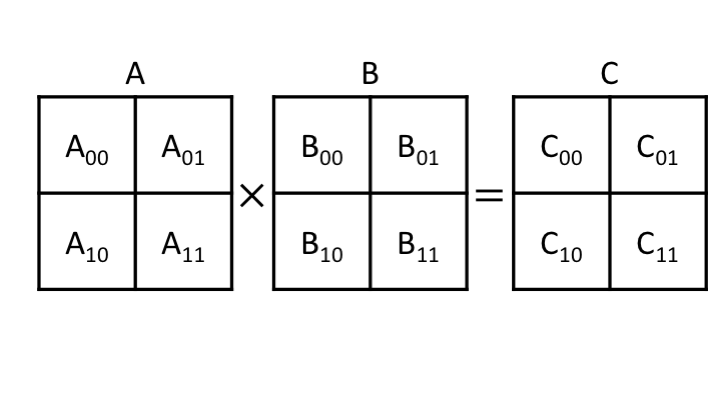
\includegraphics[width=\textwidth]{{../Figures/array_slicing/Slide18}.png}
\end{frame}

\begin{frame}[t]{Strassen's Algorithm}
	% Strassen illustration
	\centering
	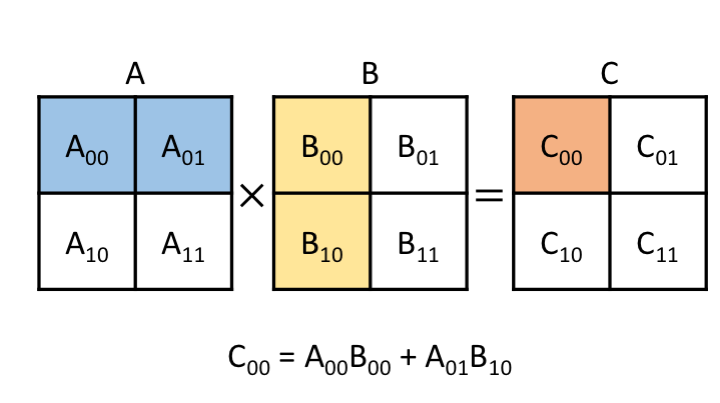
\includegraphics[width=\textwidth]{{../Figures/array_slicing/Slide19}.png}
\end{frame}

\begin{frame}[t]{Strassen's Algorithm}
	% Strassen illustration
	\centering
	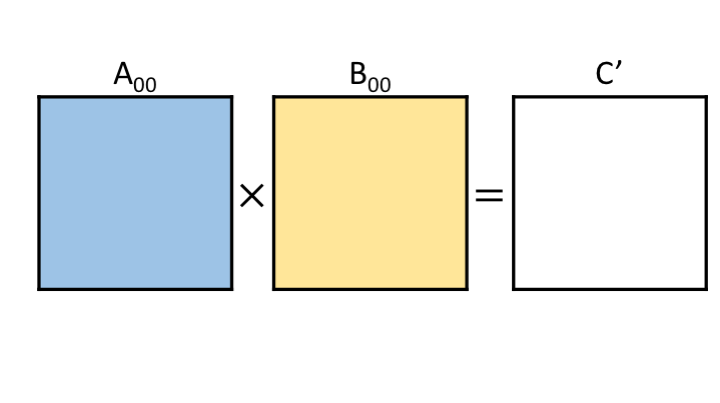
\includegraphics[width=\textwidth]{{../Figures/array_slicing/Slide20}.png}
\end{frame}

\begin{frame}[t]{Strassen's Algorithm}
	% Strassen illustration
	\centering
	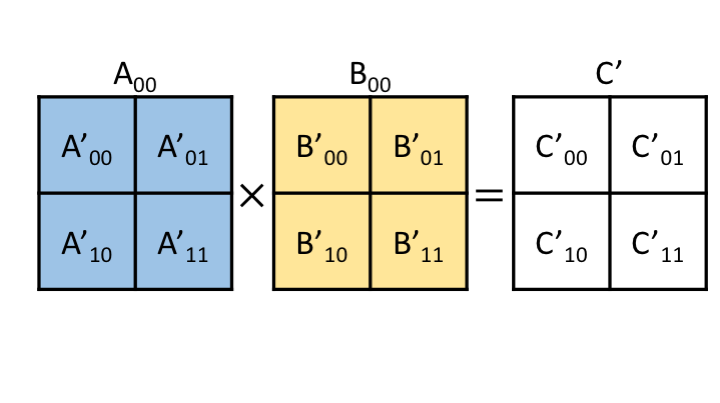
\includegraphics[width=\textwidth]{{../Figures/array_slicing/Slide21}.png}
\end{frame}

\begin{frame}[t]{Strassen's Algorithm}
	% Strassen illustration
	\centering
	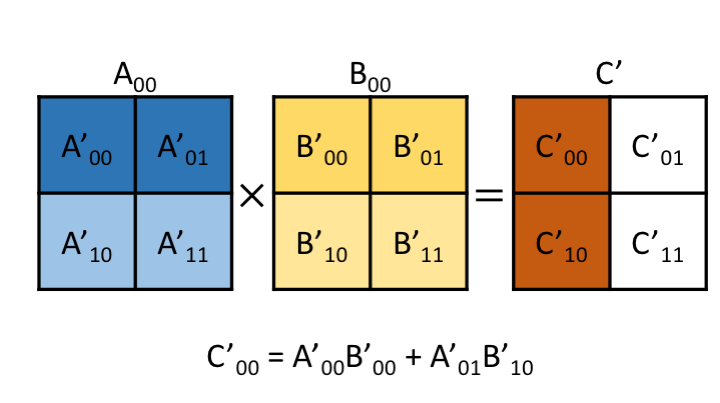
\includegraphics[width=\textwidth]{{../Figures/array_slicing/Slide22}.png}
\end{frame}

\begin{frame}[t]{Strassen's Algorithm}
	% Strassen illustration
	\begin{itemize}[<+->]
		\item Strassen's algorithm reduces the complexity of matrix multiplication from $\mathcal{O}(n^3)$ to $\approx \mathcal{O}(n^2.807)$.
		\item Many extensions to Strassen's have further reduced the complexity. Numpy uses one of these (see Demo).
		\item Strassen's is typically faster for matrices of size $100 \times 100$ and above. Good implementations will switch between naive and Strassen's.
	\end{itemize}
\end{frame}

\begin{frame}[t]{Demo}
	% Strassen Demo
	% Column Major vs. Row Major order
	\centering
	\Huge{Demo}
\end{frame}

\end{document}
